\section*{2\quad Enumeration of labeled forests by out-degree sequence.}

\noindent\textbf{Proof of Theorem 6.} For a forest $\mathbf{f}$ with vertex set $[n]$ and $i\in[n]$ let $J_i(\mathbf{f}):=\{j\in[n]: i\xrightarrow{\mathbf{f}} j\}$ be the set of children of $i$ in $\mathbf{f}$. So $\mathbf{f}$ is determined by the sequence of disjoint sets $J_1(\mathbf{f}),\ldots,J_n(\mathbf{f})$, and vice-versa. Given a sequence of disjoint subsets $J_1,\ldots,J_n$ of $[n]$, for each $m\in[n]$ let $\mathbf{f}_m$ be the relation on $[m]\cup(\bigcup_{i=1}^m J_i)$ defined by
\[
i\xrightarrow{\mathbf{f}_m} j \quad\text{iff}\quad i\in[m]\text{ and } j\in J_i. \tag{19}
\]
There exists a forest $\mathbf{f}$ labeled by $[n]$ such that $J_i(\mathbf{f})=J_i$ for all $i\in[n]$ if and only if the $J_i$ are such that $\mathbf{f}_m$ defined by (19) is a forest with vertex set $[m]\cup(\bigcup_{i=1}^m J_i)$ for every $m\in[n]$; then $\mathbf{f}=\mathbf{f}_n$ and $\mathbf{f}_m$ is the restriction of $\mathbf{f}$ to $[m]\cup(\bigcup_{i=1}^m J_i)$ for each $m\in[n]$. It follows that for each sequence of non-negative integers $(c_i)$ with $\sum_i c_i=n-k$, the number
\[
N(c_1,\ldots,c_n):=\#\{\mathbf{f}\in\mathbf{F}_{k,n}: \#J_i(\mathbf{f})=c_i \text{ for all } i\in[n]\} \tag{20}
\]
is the number of ways to choose a sequence of subsets $(J_1,\ldots,J_n)$ of $[n]$ such that $\#J_m=c_m$ and the relation $\mathbf{f}_m$ defined by (19) is a forest with vertex set $[m]\cup(\bigcup_{i=1}^m J_i)$ for every $m\in[n]$. Clearly, $J_1$ can be any of the $\binom{n-1}{c_1}$ subsets of $[n]-\{1\}$ of size $c_1$. For $m\in[n-1]$ make the inductive hypothesis that sets $J_1,\ldots,J_m$ of sizes $c_1,\ldots,c_m$ have been chosen so that $\mathbf{f}_m$ is a forest. Which choices of $J_{m+1}$ of size $c_{m+1}$ make $\mathbf{f}_{m+1}$ a forest? There are two cases to consider. Either

(i) $m+1\notin\bigcup_{i=1}^m J_i$: then $J_{m+1}$ can be any subset of $[n]-(\bigcup_{i=1}^m J_i)-\{m+1\}$;

or

(ii) $m+1\in\bigcup_{i=1}^m J_i$: then $J_{m+1}$ can be any subset of $[n]-(\bigcup_{i=1}^m J_i)-\{r_m\}$ where $r_m\notin\bigcup_{i=1}^m J_i$ is the root of the tree component of $\mathbf{f}_m$ which contains $m+1$. Either way, and regardless of what sets $J_1,\ldots,J_m$ of sizes $c_1,\ldots,c_m$ were previously chosen to make $\mathbf{f}_m$ a forest, the number of possible choices of $J_{m+1}$ which make $\mathbf{f}_{m+1}$ a forest is
\[
\binom{n-\sum_{i=1}^m c_i-1}{c_{m+1}}.
\]

Consequently, by induction
\[
N(c_1,\ldots,c_n)=\binom{n-1}{c_1}\binom{n-c_1-1}{c_2}\cdots\binom{n-\sum_{i=1}^{n-1}c_i-1}{c_n}
\]
and this expression simplifies easily to yield (15). \hfill$\square$

\section*{3\quad Enumeration of forests by type}

\noindent\textbf{Proof of Theorem 5.} Let $(n_i)$ subject to (12) be a possible type sequence for a forest of $k$ trees with $n$ vertices. According Theorem 6, for each particular sequence $(c_j)$ of type $(n_i)$ the number of forests in which $j$ has $c_j$ children for all $j\in[n]$ is
\[
\frac{k}{n}\binom{n}{k}\frac{(n-k)!}{c_1!\cdots c_n!}=\frac{k}{n}\binom{n}{k}\frac{(n-k)!}{\prod_{i\ge 0}(i!)^{n_i}}. \tag{21}
\]
But the number of sequences of non-negative integers $(c_j)$ such that $(c_j)$ has type $(n_i)$ is just the multinomial coefficient (9). The number of forests labeled by $[n]$ of type $(n_i)$ is the product of the number in (21) and this multinomial coefficient. Thus Theorem 6 implies Theorem 5, and vice versa. \hfill$\square$

\noindent\textbf{Proof of Theorem 4.} The enumeration (13) for plane forests corresponds to the enumeration (14) for labeled forests via the following map $\Psi$, which transforms a forest $\mathbf{f}$ labeled by $[n]$ into a plane forest $\Psi(\mathbf{f})$ of the same type. To define $\Psi(\mathbf{f})$, first place the components of $\mathbf{f}$ in order of their root labels, then recursively for each $g\ge 0$ place the children of each vertex of $\mathbf{f}$ at height $g$ in order of their labels. Finally, delabel to obtain the plane forest $\Psi(\mathbf{f})$. See Figure 2.

\begin{center}
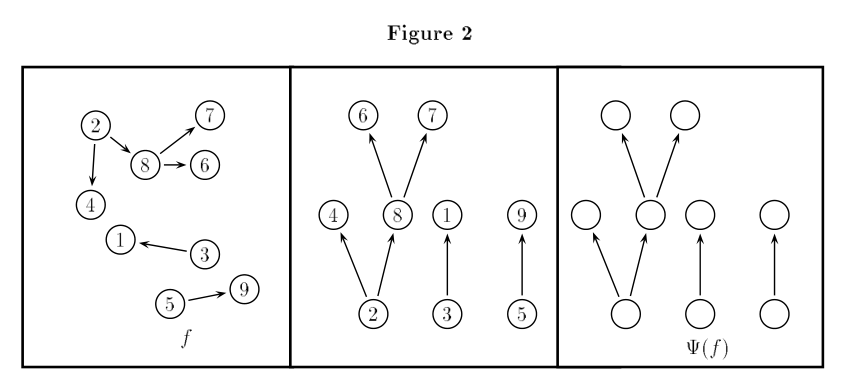
\includegraphics[width=\linewidth]{figures/pitman-tr482-figure-2.png}
\end{center}

For a fixed plane forest $\mathbf{f}^{\circ}$ with $n$ vertices and $k$ root vertices, and type $(n_i)$, let $\{v_1,\ldots,v_n\}$ be a listing of the vertices in some arbitrary order. Let $B_0$ be the set of roots of $\mathbf{f}^{\circ}$, and $B_i$ the set of children of $v_i$ for $i=1,\ldots,n$. The sets $B_i$, $0\le i\le n$, some of which must be empty, are disjoint with union $V(\mathbf{f}^{\circ})$, the set of vertices of $\mathbf{f}^{\circ}$. As discussed earlier, $V(\mathbf{f}^{\circ})$ is regarded as a subset of the set of finite sequences of positive integers. Each non-empty $B_i$ has a linear ordering, and each $\mathbf{f}\in\Psi^{-1}(\mathbf{f}^{\circ})$ corresponds to a unique bijection from $V(\mathbf{f}^{\circ})$ to $[n]$ which is increasing on each non-empty $B_i$. It follows that $\#\Psi^{-1}(\mathbf{f}^{\circ})$, the number of forests $\mathbf{f}$ labeled by $[n]$ such that $\Psi(\mathbf{f})=\mathbf{f}^{\circ}$ is the multinomial coefficient
\[
\#\Psi^{-1}(\mathbf{f}^{\circ})=\binom{n!}{k,\#B_1,\ldots,\#B_n}=\frac{n!}{k!\prod_{v\in V(\mathbf{f}^{\circ})} C(v,\mathbf{f}^{\circ})!}=\frac{n!}{k!\prod_{i\ge 0}(i!)^{n_i}} \tag{22}
\]
where $C(v,\mathbf{f}^{\circ})$ is the number of children of $v$ in the forest $\mathbf{f}^{\circ}$, and $(n_i)$ is the type of $\mathbf{f}^{\circ}$ and of every $\mathbf{f}\in\Psi^{-1}(\mathbf{f}^{\circ})$. It follows that the number $N^{\mathit{plane}}(n_0,n_1,\ldots)$ of plane forests of type $(n_i)$ and the corresponding number $N^{[n]}(n_0,n_1,\ldots)$ of forests of type $(n_i)$ labeled by $[n]$ are related by
\[
\frac{N^{[n]}(n_0,n_1,\ldots)}{N^{\mathit{plane}}(n_0,n_1,\ldots)}=\frac{n!}{k!\prod_{i\ge 0}(i!)^{n_i}}. \tag{23}
\]
Hence the equivalence of Theorems 4 and 5. \hfill$\square$

\section*{4\quad The Otter-Dwass formula}

\noindent\textbf{Proof of the equivalence of Theorems 1 and 4.} Following Otter [43] and subsequent authors [30, 37, 13], regard a Galton-Watson process started with $Z_0=k$ individuals as generating a collection of $k$ family trees, which combine to form a random family forest $\mathcal{F}_k$. On the event $(\#\mathcal{F}_k<\infty)$ the random family forest $\mathcal{F}_k$ can be defined in an elementary way as a random element with values in the countable set $\mathbf{F}$ of all plane forests. The distribution of $\mathcal{F}_k$ is then the sub-probability distribution on $\mathbf{F}$ defined by the formula [43]
\[
P(\mathcal{F}_k=\mathbf{f})=\prod_{v\in V(\mathbf{f})} p_{C(v,\mathbf{f})}=\prod_{i\ge 0} p_i^{n_i(\mathbf{f})} \quad \forall k\ge 1,\ \mathbf{f}\in\mathbf{F}_k^{\mathit{plane}} \tag{24}
\]
where $V(\mathbf{f})$ is the set of vertices of $\mathbf{f}$, the number of vertices of $\mathbf{f}$ with $i$ children is denoted $n_i(\mathbf{f})$, and $\mathbf{F}_k^{\mathit{plane}}$ is the set of plane forests with $k$ root vertices. This distribution on $\mathbf{F}_k^{\mathit{plane}}$ has total mass $P(\#\mathcal{F}_k<\infty)\le 1$. For each $k=1,2,\ldots$ the probability of the event $(\#\mathcal{F}_k=n)$ is obtained by summing the expression (24) over all plane forests $\mathbf{f}$ of $k$ trees with a total of $n$ vertices. The terms in this sum can be classified by the type $(n_i)$ of the forest $\mathbf{f}$. Since the number of vertices in a forest of type $(n_i)$ is $\sum_i n_i$ and the number of root vertices is $n-\sum_i n_i$, the result is
\[
P(\#\mathcal{F}_k=n)=\sum_{\substack{\Sigma n_i=n\\ \Sigma i n_i=n-k}} N^{\mathit{plane}}(n_0,n_1,\ldots)\prod_{i\ge 0} p_i^{n_i} \tag{25}
\]
where the sum is over all possible types of a sequence with length $n$ and sum $n-k$. Now fix $n$ and $k$ and regard the probability displayed in (25), and the probability $P(S_n=m)$ displayed in (8) for $m=n-k$, as functions of the sequence $(p_0,\ldots,p_n)$. Since each probability is a polynomial in $(p_0,\ldots,p_n)$, the Otter-Dwass formula (4) is an identity of polynomials whose coefficient identity is the enumeration (13) of plane forests by type. \hfill$\square$
